\documentclass[10pt]{beamer}

%% \usetheme[progressbar=foot]{metropolis}
\newcommand{\metroset}[1]{}

% Pour plusieurs pages par feuille dans les handout
% \usepackage{pgfpages}
% \pgfpagesuselayout{4 on 1}[a4paper,border shrink=3mm, landscape]
\usetheme{Antibes}                        % Beamer theme v 3.0
\usecolortheme{dolphin}                   % Beamer color theme

% -------------------------------------------------------------------------
% Style

% nice colors %%%%%%%%%%%%%%%%%%%%%%%%%%%%%%%%%%%%%%%%%%%%%%%%%%
\definecolor{niceblue}{HTML}{4747ba}
\definecolor{blue}{HTML}{4747ba} %!!!!!! section courante en haut
\definecolor{nicegreen}{HTML}{6C9034}
\definecolor{nicered}{HTML}{b02323}
% blocks (example blocks and simple blocks) %%%%%%%%%%%%%%%%%%%%
\setbeamertemplate{blocks}[rounded]

%% \setbeamercolor{block title example}{fg=white,bg=nicegreen}
%% %\setbeamercolor{block body example}{fg=black,bg=nicegreen!10!white}
%% %change tout seul avec le style du titre

%% \setbeamercolor{block title}{fg=blue,bg=niceblue!20!white}%fg=white,bg=niceblue}
%% \setbeamercolor{block body}{fg=black,bg=niceblue!20!white}
%% \setbeamerfont{block title}{size=\small,series=\bfseries}

\setbeamercolor{block title alerted}{fg=white,bg=red!20!white}
\setbeamercolor{block body alerted}{fg=black,bg=white}

%% % \setbeamercovered{transparent} % texte caché devient visible (grisé)

\setbeamercolor{alerted text}{fg=nicered}
\setbeamercolor{example text}{fg=nicegreen!95!black}

%\beamertemplateballitem
%\beamertemplatenumberedballsectiontoc
\usenavigationsymbolstemplate{}           % To remove navigation symbols

\setbeamertemplate{sections/subsections in toc}[default]
\setbeamertemplate{itemize items}[default]
\setbeamercolor{itemize item}{fg=niceblue!55!white}
\setbeamercolor{itemize subsubitem}{fg=lightgray}

% entête et pied des slides %%%%%%%%%%%%%%%%%%%%%%%%%%%%%%%%%%%%
\useoutertheme{infolines} %principalement pour pouvoir utiliser toute la largeur
                          % des slides car l'entête est redéfinie ensuite
\setbeamercolor{section in head/foot}{fg=niceblue,bg=white}

\setbeamertemplate{footline}{             % pied des slides
  \begin{beamercolorbox}[wd=\paperwidth,ht=2.25ex,dp=1ex,right]{}
    \insertframenumber/\inserttotalframenumber\ \
  \end{beamercolorbox}
}
\setbeamertemplate{headline}{             % entête des slides
  \begin{beamercolorbox}[wd=\paperwidth,ht=2.25ex,dp=1ex,left]{}%
    \insertsectionnavigationhorizontal{\paperwidth}{}{}
  \end{beamercolorbox}
  \vspace{-0.1cm}
}

%\setbeamercolor{button}{bg=nicered!20!white,fg=black}
%\setbeamercolor{button border}{fg=nicered!20!white}
%\setbeamerfont{button}{size=\normalsize}

\renewcommand{\emph}[1]{{\usebeamercolor[fg]{title}{#1}}} % niceblue
\newcommand{\green}[1]{{\usebeamercolor[fg]{example text}{#1}}}  % dark nicegreen
\renewcommand{\cite}[1]{{\color{brown}{[#1]}}}


\usepackage{appendixnumberbeamer}
\usepackage{booktabs}
%% \usepackage[scale=2]{ccicons}
\usepackage{tikz-cd} 
\usepackage{hyperref}
\usepackage{mathtools}
\usepackage{quiver}
\usepackage{stackengine,scalerel}
\newcommand\eye{\ensurestackMath{\stackinset{c}{}{c}{-.33pt}%
		{\bullet}{\bigcirc}}}
\usepackage{graphicx} % Allows including images
\usepackage{bussproofs}
\usepackage{tikz}
\usetikzlibrary{cd}
\usepackage{adjustbox}
\usetikzlibrary{petri,positioning}
\usepackage{booktabs} % Allows the use of \toprule, \midrule and \bottomrule in tables

\usepackage{pgfplots}
\usepgfplotslibrary{dateplot}

\definecolor{lightblue} {rgb}{.75,.85,1}
\definecolor{blk}    {rgb}{0,0,0}
\definecolor{red}    {rgb}{.8,0,0}
\definecolor{green}  {rgb}{0,.7,0}
%% \definecolor{blue}   {rgb}{0,0,.9}
\definecolor{blue}   {HTML}{4747ba}
\definecolor{brown}  {rgb}{.6,.3,0}
\definecolor{yellow} {rgb}{0.9,0.9,0.5}
\definecolor{gray}  {rgb}{.8,.8,.8}
\definecolor{darkgray}  {rgb}{.6,.6,.6}
\newcommand<>\blk[1] {{\color#2{blk}#1}}
\newcommand<>\red[1] {{\color#2{red}#1}}
%% \newcommand<>\blu[1] {{\color#2{blue}#1}}
\newcommand<>\blu[1] {\blue{#1}}
\newcommand<>\grn[1] {{\color#2{green}#1}}
\newcommand<>\brw[1] {{\color#2{brown}#1}}
\newcommand<>\yel[1] {{\color#2{yellow}#1}}
\newcommand<>\gray[1] {{\color#2{gray}#1}}
\newcommand<>\darkgray[1] {{\color#2{darkgray}#1}}
\definecolor{niceblue}{HTML}{4747ba}
\newcommand{\blue}[1]{\textcolor{niceblue}{#1}}
\newcommand{\white}{\color{white}\footnotesize}
\newcommand{\sequence}[1]{\ensuremath \langle #1 \rangle}
\newcommand{\logs}	{\blu L}
\newcommand{\sys}		{\mathcal{\blu S}}
\newcommand{\model}	{\blu N}
\newcommand{\Tab}[2]{\begin{tabular}{@{}#1@{}}#2\end{tabular}}
\newcommand{\Tabt}[2]{\begin{tabular}[t]{@{}#1@{}}#2\end{tabular}}
\newcommand{\Ar}[2]{\ensuremath{\begin{array}{@{}#1@{}}#2\end{array}}}
\newcommand{\Arrayt}[2]{\ensuremath{\begin{array}[t]{@{}#1@{}}#2\end{array}}}
\newcommand{\mathdef}[1]{\stackrel{\text{\tiny \ensuremath{\mi{def}}}}{#1}}
\newcommand{\define}{\mathdef{=}}
\newcommand{\iffdef}{\mathdef{\iff}}
\newcommand{\Language} {\mathcal{L}}
\newcommand{\dist} {\mathit{dist}}
\newcommand{\toolAntialignments} {\textsc{DarkSider}}
\newcommand{\toolMultialignments} {\textsc{DarkSider}}


\usepackage{xspace}
\newcommand{\themename}{\textbf{\textsc{metropolis}}\xspace}

\title{Towards Conformance Checking for\\ Timed Process Models}
%\subtitle{A modern beamer theme}
% \date{\today}
\date{}
\author[author] {{\large Thomas Chatain}\\ joint work with Neha Rino}
\institute{LMF, ENS Paris-Saclay}
% \titlegraphic{\hfill\includegraphics[height=1.5cm]{logo.pdf}}

\begin{document}

\maketitle


\section[Introduction]{Introduction}
\begin{frame}{Process Mining}
  \begin{columns}
    \begin{column}{.4\textwidth}
      Young and very active research domain\medskip\\
      At the interface between
    \begin{itemize}
    \item Data science
    \item Formal methods
    \end{itemize}
    \medskip
    \end{column}
    \begin{column}{.5\textwidth}
      \scalebox{.5}{
        \begin{tabular}{|c|c|c|c|c|c|}
          \hline
          patient & activity & timestamp & doctor & age & cost\\\hline\hline
          5781 & make X-ray & 23-1-2014:10.30 & Dr. Jones & 45 & 70.00\\
          5541 & blood test & 23-1-2014:10.18 & Dr. Scott & 61 & 40.00\\
          5833 & blood test & 23-1-2014:10.27 & Dr. Scott & 24 & 40.00\\
          5781 & blood test & 23-1-2014:10.49 & Dr. Scott & 45 & 40.00\\
          5781 & CT scan & 23-1-2014:11.10 & Dr. Fox & 45 & 1200.00\\
          5833 & surgery & 23-1-2014:12.34 & Dr. Scott & 24 & 2300.00\\
          5781 & handle payment & 23-1-2014:12.41 & Carol Hope & 45 & 0.00\\
          5541 & radiation therapy & 23-1-2014:13.57 & Dr. Jones & 61 & 140.00\\
          5541 & radiation therapy & 23-1-2014:13.08 & Dr. Jones & 61 & 140.00\\
          \hline
        \end{tabular}
      }
    \end{column}
  \end{columns}
  \bigskip\pause

  \begin{block}{Discovery and analysis of process models from real process executions}
    \begin{itemize}
    \item analyze usage of an e-commerce web site
    \item analyze medical processes in hospitals
    \item improve user interface
    \item detect deviant behavior
    \end{itemize}
  \end{block}
  \bigskip
  Many (Industrial) Process Mining Tools
  \begin{itemize}
  \item Celonis, Disco, Minit, ProM, PM4PY\dots
  \end{itemize}
\end{frame}

%% \emph{Output:} Process Models\\
%% 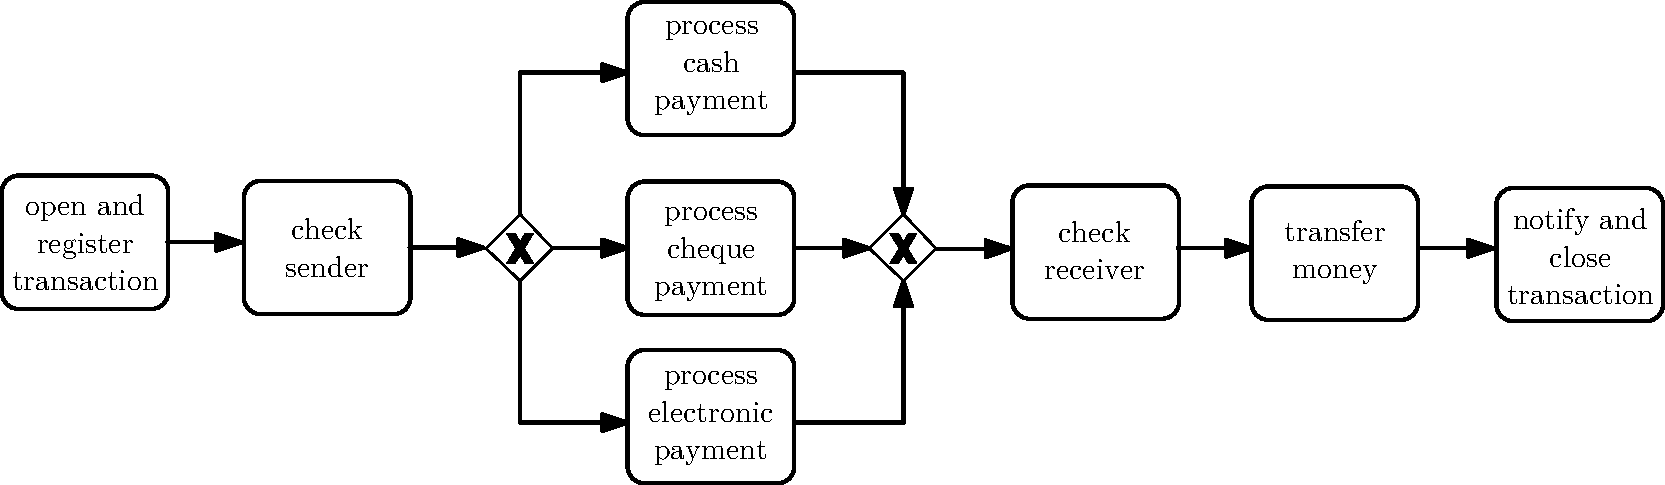
\includegraphics[width=.6\textwidth]{runningstructure.pdf}.

\begin{frame}{Event Logs and Data Extraction\footnote{Acknowledgements to Wil van der Aalst}}
  \only<1>{
  \begin{tabular}{|c|c|c|c|c|c|}
    \hline
    patient & activity & timestamp & doctor & age & cost\\\hline\hline
    5781 & make X-ray & 23-1-2014:10.30 & Dr. Jones & 45 & 70.00\\
    5541 & blood test & 23-1-2014:10.18 & Dr. Scott & 61 & 40.00\\
    5833 & blood test & 23-1-2014:10.27 & Dr. Scott & 24 & 40.00\\
    5781 & blood test & 23-1-2014:10.49 & Dr. Scott & 45 & 40.00\\
    5781 & CT scan & 23-1-2014:11.10 & Dr. Fox & 45 & 1200.00\\
    5833 & surgery & 23-1-2014:12.34 & Dr. Scott & 24 & 2300.00\\
    5781 & handle payment & 23-1-2014:12.41 & Carol Hope & 45 & 0.00\\
    5541 & radiation therapy & 23-1-2014:13.57 & Dr. Jones & 61 & 140.00\\
    5541 & radiation therapy & 23-1-2014:13.08 & Dr. Jones & 61 & 140.00\\
    \hline
  \end{tabular}
}
  \only<2>{
  \begin{tabular}{|c|c|c|}
    \hline
    patient & activity & timestamp\\\hline\hline
    5781 & make X-ray & 23-1-2014:10.30 \\
    5541 & blood test & 23-1-2014:10.18 \\
    5833 & blood test & 23-1-2014:10.27 \\
    5781 & blood test & 23-1-2014:10.49 \\
    5781 & CT scan    & 23-1-2014:11.10 \\
    5833 & surgery    & 23-1-2014:12.34 \\
    5781 & handle payment    & 23-1-2014:12.41\\
    5541 & radiation therapy & 23-1-2014:13.57\\
    5541 & radiation therapy & 23-1-2014:13.08\\
    \hline
  \end{tabular}
}
  \only<3>{
  \begin{tabular}{|c|c|c|}
    \hline
    patient & activity & timestamp \\\hline\hline
    \red{5781} & make X-ray   & 23-1-2014:10.30 \\
    \blue{5541} & blood test  & 23-1-2014:10.18 \\
    \green{5833} & blood test & 23-1-2014:10.27 \\
    \red{5781} & blood test   & 23-1-2014:10.49 \\
    \red{5781} & CT scan      & 23-1-2014:11.10 \\
    \green{5833} & surgery    & 23-1-2014:12.34 \\
    \red{5781} & handle payment     & 23-1-2014:12.41 \\
    \blue{5541} & radiation therapy & 23-1-2014:13.57 \\
    \blue{5541} & radiation therapy & 23-1-2014:13.08 \\
    \hline
  \end{tabular}
}
  \only<4>{
  \begin{tabular}{|c|c|c|}
    \hline
    patient & activity & timestamp \\\hline\hline
    \red{5781} & make X-ray         & 23-1-2014:10.30\\
    \red{5781} & blood test         & 23-1-2014:10.49\\
    \red{5781} & CT scan            & 23-1-2014:11.10\\
    \red{5781} & handle payment     & 23-1-2014:12.41\\
    \hline
    \blue{5541} & blood test        & 23-1-2014:10.18\\
    \blue{5541} & radiation therapy & 23-1-2014:13.57\\
    \blue{5541} & radiation therapy & 23-1-2014:13.08\\
    \hline
    \green{5833} & blood test       & 23-1-2014:10.27\\
    \green{5833} & surgery          & 23-1-2014:12.34\\
    \hline
  \end{tabular}
}
  \only<5>{
  \begin{tabular}{|c|c|c|}
    \hline
    patient & activity & timestamp \\\hline\hline
    \white{5781} & make X-ray        &\\
    \white{5781} & blood test        &\\
    \white{5781} & CT scan           &\\
    \white{5781} & handle payment    &\\
    \hline
    \white{5541} & blood test        &\\
    \white{5541} & radiation therapy &\\
    \white{5541} & radiation therapy &\\
    \hline
    \white{5833} & blood test        &\\
    \white{5833} & surgery           &\\
    \hline
  \end{tabular}
}
  \only<6->{
  \begin{tabular}{|c|c|c|}
    \hline
    patient & activity & timestamp \\\hline\hline
    & X & \\
    & B & \\
    & C & \\
    & P & \\
    \hline
    & B & \\
    & R & \\
    & R & \\
    \hline
    & B & \\
    & S & \\
    \hline
  \end{tabular}
}
  \only<7>{\bigskip\\
    $\sequence{X, B, C, P}$\\
    $\sequence{B, R, R}$\\
    $\sequence{B, S}$\\
}
\end{frame}

%% \section{Process Discovery}
\begin{frame}{Process Discovery}
  \begin{block}{}
    Automatic construction of a
    %% ``representative'' system
    model $\model$ from an event log $\logs$ that represents a
    partial observation of a system $\sys$.
  \end{block}
  \bigskip
  \bigskip
  \pause

  \begin{tabular}{c}
    \scalebox{.7}{
      \begin{tabular}{l}
        $\langle A,B,D,E,I \rangle$    \\
        $\langle A,C,D,G,H,F,I \rangle$  \\
        $\langle A,C,G,D,H,F,I \rangle$  \\
        $\langle A,C,H,D,F,I \rangle$    \\
        $\langle A,C,D,H,F,I \rangle$    \\
      \end{tabular}
    }\medskip\\
    \emph{\(L\)}
  \end{tabular}
  \hfill\pause\(\longrightarrow\)\hfill
  \raisebox{0cm}{
    \begin{tabular}{c}
      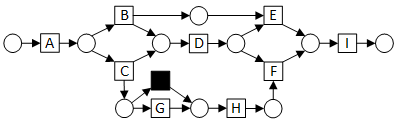
\includegraphics[width=5cm]{model_Boudewijn.png}\medskip\\
      \emph{\(N\)}
    \end{tabular}
  }
\end{frame}

\begin{frame}{Process Discovery: Several Solutions}
  \bigskip

  \raisebox{.5cm}{Log: \(\Ar{l}{
      \sequence{A,B,D,E,I}\\
      \sequence{A,C,D,G,H,F,I}\\
      \sequence{A,C,G,D,H,F,I}\\
      \sequence{A,C,H,D,F,I}\\
      \sequence{A,C,D,H,F,I}\\
    }\)}
  \hfill
  \Tab{c}{\small
    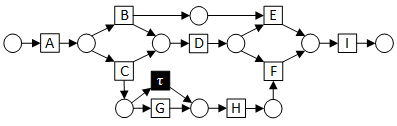
\includegraphics[scale=.5]{fig_BPM/Model_1.png}\\
  }\bigskip\\
  \Tab{c}{\small
    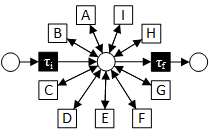
\includegraphics[scale=.5]{fig_BPM/Model_3.png}\\
  }\hfill
  \Tab{c}{\small
    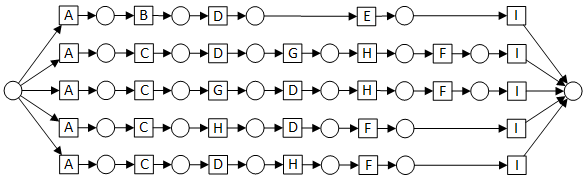
\includegraphics[scale=.5]{fig_BPM/Model_4.png}\\
  }
\end{frame}


\section{Conformance Checking}
\begin{frame}{Conformance Checking}
  \scalebox{.7}{\begin{tabular}{l}
    $\langle A,B,D,E,I \rangle$    \\
    $\langle A,C,D,G,H,F,I \rangle$  \\
    $\langle A,C,G,D,H,F,I \rangle$  \\
    $\langle A,C,H,D,F,I \rangle$    \\
    $\langle A,C,D,H,F,I \rangle$    \\
  \end{tabular}}
  \hfill\(\longrightarrow\)\hfill
  \raisebox{-.8cm}{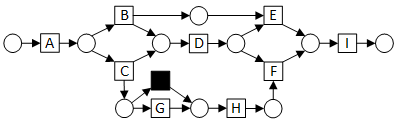
\includegraphics[width=5cm]{model_Boudewijn.png}}
  \\\pause\hspace*{0.8\textwidth}{\Huge ?}
  \bigskip
  \pause

  \begin{block}{Define quality criteria to evaluate models}
    \begin{itemize}
    \item $\model$ \emph{fits} $\logs$ if $\logs \subseteq \Language(\model)$
    \item $\model$ is \emph{precise} if its runs are \textit{close} to traces of $\logs$
    \item $\model$ \emph{generalizes} $\logs$ %% with respect to ${\sys}$
      if $\Language(\model)$ contains some unobserved behavior $\not\in
      %% in $\Language(\sys) \backslash
      \logs$
    \item \emph{simplicity}\dots
    \end{itemize}
  \end{block}
\end{frame}

\begin{frame}{Conformance Checking: Example}
  \bigskip

  \raisebox{.5cm}{Log: \(\Ar{l}{
      \sequence{A,B,D,E,I}\\
      \sequence{A,C,D,G,H,F,I}\\
      \sequence{A,C,G,D,H,F,I}\\
      \sequence{A,C,H,D,F,I}\\
      \sequence{A,C,D,H,F,I}\\
    }\)}
  \hfill
  \Tab{c}{\small
    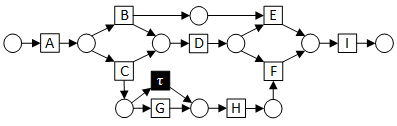
\includegraphics[scale=.5]{fig_BPM/Model_1.png}\\
    \uncover<3->{
      \green{fitting}\\
      \green{fairly precise}\\
      \green{simple}\\
      \green{generalizing}}}\bigskip\\
  \Tab{c}{\small
    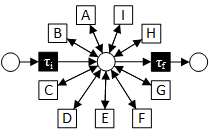
\includegraphics[scale=.5]{fig_BPM/Model_3.png}\\
    \uncover<4->{
      \green{fitting}\\
      \red{very imprecise}\\
      \green{simple}\\
      \green{generalizing}}}\hfill
  \Tab{c}{\small
    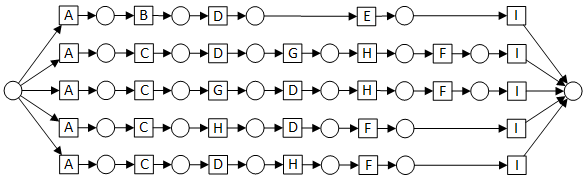
\includegraphics[scale=.5]{fig_BPM/Model_4.png}\\
    \uncover<5->{
      \green{fitting}\\
      \green{very precise}\\
      \red{not simple}\\
      \red{not generalizing}}}
\end{frame}




\begin{frame}{Alignments}

\emph{Estimating fitness}
\bigskip

  \raisebox{.5cm}{Log: \(\Ar{l}{
      \sequence{A,B,D,E,I}\\
      \sequence{A,C,D,G,H,F,I}\\
      \sequence{A,C,G,D,H,F,I}\\
      \sequence{A,C,H,D,F,I}\\
      \sequence{A,C,D,H,F,I}\\
      \sequence{A,B,D,G,H,F,I}\\
    }\)}
  \hfill
    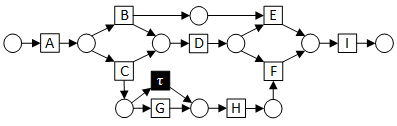
\includegraphics[scale=.5]{fig_BPM/Model_1.png}\bigskip\\
    %% \emph{Example:}\\
    \begin{tabular}{ll}
      Trace & \(\sigma = \sequence{A,B,D,G,H,F,I}\)\\
      \uncover<3->{Alignment: & \(\gamma = \sequence{A,\alert{C},D,G,H,F,I}\)}
    \end{tabular}
    \pause
\begin{block}{Alignment}
  Given a trace $\sigma$ and a model \(N\),\\
  an alignment is a full run $\gamma$ of \(N\) which minimizes its
  (Levenshtein) distance to $\sigma$.

  %% If $\model$ \emph{fits} $\logs$, then $\gamma = \sigma$.
\end{block}

\bigskip\pause\pause
\emph{Central notion in conformance checking}
\end{frame}

%% %\begin{frame}[fragile]{Day One}

%% %	 \includegraphics[width=0.2\textwidth]{employee.png}
%% %	 \hspace{1.5em}
%% %%	 	\includegraphics[width= 0.5\textwidth]{airline.jpg}
%% %\end{frame}

%% \begin{frame}[fragile]{An example}

%% \centerline{
%% 	\begin{tabular}{|c| c| c| c|}
%% 		\hline
%% 		Emp ID & Action & Customer ID & timestamp \\ 
%% 		\hline
%% 		1 & reg & 70 & 13:31\\
%% 		2 & reg & 71 & 13:32\\
%% 		1 &et & 70 & 13:32\\
%% 		1& ct & 70 & 13:33\\
%% 		2& reg & 72 & 13:34\\
%% 		2& ec & 71 & 13:34\\
%% 		\hline
%% 	\end{tabular}
%% }
%% \vfill 
%% Register request : reg, Examine thoroughly : et, Examine casually : ec, Check ticket : ct, Decide : dec, Pay : pay, and Reject : rej. 

%% \end{frame}
%% \begin{frame}
%% 	Group by customer ID, throw away other details : 
%% 	\vfill 
	
%% 	\centerline{
%% 		\begin{tabular}{|c| c| }
%% 			\hline
%% 			Customer ID & Action \\ 
%% 			\hline
%% 			70 &  reg \\
%% 			70 & et \\
%% 			70 & ct \\
%% 			70 & dec \\
%% 			70 & pay \\
%% 			\hline
%% 			71 & reg \\
%% 			71 & ec \\
%% 			71 & ct \\
%% 			71 & dec\\
%% 			71 & rej \\
%% 			\hline
%% 			72 & reg\\
%% 			72&ct\\
%% 			\hline
%% 		\end{tabular}
%% 	}
	
%% \end{frame}


%% \begin{frame}[fragile]{Process Mining}

%% Perhaps, we deduce the following process model : \vfill 
%% \adjustbox{scale=0.7}{
%% 	\begin{tikzcd}
%% 		&& {\Huge{\bigcirc}} & {\fbox{et}} & {\Huge{\bigcirc}} &&& {\fbox{pay}} \\
%% 		{\Huge{\bigcirc}} & {\fbox{reg}} && {\fbox{ec}} && {\fbox{dec}} & {\Huge{\bigcirc}} && {\Huge{\bigcirc}} \\
%% 		&& {\Huge{\bigcirc}} & {\fbox{ct}} & {\Huge{\bigcirc}} &&& {\fbox{rej}}\\
%% 		\arrow[from=2-1, to=2-2]
%% 		\arrow[curve={height=-12pt}, from=2-2, to=1-3]
%% 		\arrow[curve={height=12pt}, from=2-2, to=3-3]
%% 		\arrow[from=1-3, to=1-4]
%% 		\arrow[from=1-4, to=1-5]
%% 		\arrow[from=3-3, to=3-4]
%% 		\arrow[from=3-4, to=3-5]
%% 		\arrow[curve={height=12pt}, from=3-5, to=2-6]
%% 		\arrow[curve={height=-12pt}, from=1-5, to=2-6]
%% 		\arrow[from=2-6, to=2-7]
%% 		\arrow[curve={height=-12pt}, from=2-7, to=1-8]
%% 		\arrow[curve={height=12pt}, from=2-7, to=3-8]
%% 		\arrow[curve={height=12pt}, from=1-3, to=2-4]
%% 		\arrow[curve={height=12pt}, from=2-4, to=1-5]
%% 		\arrow[curve={height=-12pt}, from=1-8, to=2-9]
%% 		\arrow[curve={height=12pt}, from=3-8, to=2-9]
%% 	\end{tikzcd}
%% }


%% \end{frame}

\begin{frame}{Timestamps}
	But sometimes, we want to retain the timing information :   
	\vfill 
	
	\centerline{
	\begin{tabular}{|c| c| c|}
		\hline
		Customer ID & Action & timestamp \\ 
		\hline
		70 &  reg & 13:31\\
		70 & et & 13:32\\
		70 & ct & 13:33\\
		70 & dec & 13:37\\
		70 & pay & 13:38\\
		\hline
		71 & reg & 13:32\\
		71 & ec & 13:34\\
		71 & ct & 13:34\\
		71 & dec & 13:36\\
		71 & rej & 13:36\\
		\hline
		72 & reg & 13:34\\
		72 & ct & 13:36\\
		\hline
	\end{tabular}
}

	
\end{frame}
\begin{frame}[fragile]{Time Constraints : Time Petri Nets}
Now, maybe we could have a process model like : 
\vfill 
\adjustbox{scale=0.7}{
\begin{tikzcd}
	& {} & \Huge\bigcirc & {\fbox{ec}} & \Huge\bigcirc & {} && {\fbox{pay}} \\
	\Huge\bigcirc & {\fbox{reg}} && {\fbox{et}} && {\fbox{dec}} & \Huge\bigcirc & {} & \Huge\bigcirc \\
	&& \Huge\bigcirc & {\fbox{ct}} & \Huge\bigcirc &&& {\fbox{rej}}
	\arrow["{[0, \infty]}"{description, pos=0.2}, shift left=3, draw=white, from=2-2, to=1-2]
	\arrow[""{name=0, anchor=center, inner sep=0}, "{[2,2]}"{description, pos=0.1}, draw=white, from=2-4, to=1-4]
	\arrow["{[2,2]}"{description, pos=0.1}, draw=white, from=3-4, to=2-4]
	\arrow["{[2,4]}"{description, pos=0.1}, shift right=4, draw=white, from=2-6, to=1-6]
	\arrow["{[0,1]}"{description, pos=0.1}, draw=white, from=1-8, to=2-8]
	\arrow["{[0,0]}"{description, pos=0.1}, draw=white, from=3-8, to=2-8]
	\arrow[from=2-1, to=2-2]
	\arrow[curve={height=-12pt}, from=2-2, to=1-3]
	\arrow[curve={height=12pt}, from=2-2, to=3-3]
	\arrow[from=1-3, to=1-4]
	\arrow[from=1-4, to=1-5]
	\arrow[curve={height=12pt}, from=1-3, to=2-4]
	\arrow[curve={height=12pt}, from=2-4, to=1-5]
	\arrow[from=3-3, to=3-4]
	\arrow[from=3-4, to=3-5]
	\arrow[curve={height=-12pt}, from=1-5, to=2-6]
	\arrow[curve={height=12pt}, from=3-5, to=2-6]
	\arrow[from=2-6, to=2-7]
	\arrow[curve={height=-12pt}, from=2-7, to=1-8]
	\arrow[curve={height=12pt}, from=2-7, to=3-8]
	\arrow[curve={height=12pt}, from=3-8, to=2-9]
	\arrow[curve={height=-12pt}, from=1-8, to=2-9]
	\arrow["{[0,2]}"{description, pos=0.2}, draw=white, from=1-4, to=0]
\end{tikzcd}
}
\end{frame}

%% %\begin{frame}[fragile]{Processes, Event Logs and Models}
	
%% %\huge{$$Model \xLeftrightarrow[Checking]{Conformance}  Event Log$$}
	
%% %\end{frame}


%% \subsection{Conformance Checking}

%% \begin{frame}{Conformance Checking}
%%     \begin{itemize}
%%         \item Relating observed and modelled behaviour [CarmonaDSW18]
%%         \vfill 
%%         \item Evaluate a process model, or correct an event log using precision, fitness, simplicity, generalisation, etc
%%         \vfill 
%%         \item Fitness : Does model represent the process well? 

%%     \end{itemize}
%%         \vfill 
%% $$Log \subseteq \mathcal{L}(N)$$
%% \end{frame}

%% \begin{frame}[fragile]{Alignments}
%%   \emph{Estimating fitness}
%%   \bigskip

%% \begin{block}{Alignment}
%%   Given a trace $\sigma$ and a model \(N\),\\
%%   an alignment is a full run $\gamma$ of \(N\) which minimizes its
%%   distance to $\sigma$.

%%   %% If $\model$ \emph{fits} $\logs$, then $\gamma = \sigma$.
%% \end{block}

%%   \adjustbox{scale=0.7}{
%% 		\begin{tikzcd}
%% 			&& {\Huge{\bigcirc}} & {\fbox{et}} & {\Huge{\bigcirc}} &&& {\fbox{pay}} \\
%% 			{\Huge{\bigcirc}} & {\fbox{reg}} && {\fbox{ec}} && {\fbox{dec}} & {\Huge{\bigcirc}} && {\Huge{\bigcirc}} \\
%% 			&& {\Huge{\bigcirc}} & {\fbox{ct}} & {\Huge{\bigcirc}} &&& {\fbox{rej}}\\
%% 			\arrow[from=2-1, to=2-2]
%% 			\arrow[curve={height=-12pt}, from=2-2, to=1-3]
%% 			\arrow[curve={height=12pt}, from=2-2, to=3-3]
%% 			\arrow[from=1-3, to=1-4]
%% 			\arrow[from=1-4, to=1-5]
%% 			\arrow[from=3-3, to=3-4]
%% 			\arrow[from=3-4, to=3-5]
%% 			\arrow[curve={height=12pt}, from=3-5, to=2-6]
%% 			\arrow[curve={height=-12pt}, from=1-5, to=2-6]
%% 			\arrow[from=2-6, to=2-7]
%% 			\arrow[curve={height=-12pt}, from=2-7, to=1-8]
%% 			\arrow[curve={height=12pt}, from=2-7, to=3-8]
%% 			\arrow[curve={height=12pt}, from=1-3, to=2-4]
%% 			\arrow[curve={height=12pt}, from=2-4, to=1-5]
%% 			\arrow[curve={height=-12pt}, from=1-8, to=2-9]
%% 			\arrow[curve={height=12pt}, from=3-8, to=2-9]
%% 		\end{tikzcd}
%% 	}

%% 	\begin{itemize}
%% 		\item Observed trace: \alert{$\sigma = reg \cdot et \cdot et \cdot ct \cdot dec \cdot pay$} 
%% 		\vfill 
%% 		\item Optimal alignment: \alert{$\gamma = reg \cdot et \cdot ct \cdot dec \cdot pay$}
%% 	\end{itemize}

%%         \bigskip\pause\pause
%%         \emph{Central notion in conformance checking}

%% \end{frame}


\begin{frame}[fragile]{Timed Alignments}
  \emph{Now suppose we keep the timestamps}
\adjustbox{scale=0.7}{
\begin{tikzcd}
	& {} & \Huge\bigcirc & {\fbox{ec}} & \Huge\bigcirc & {} && {\fbox{pay}} \\
	\Huge\bigcirc & {\fbox{reg}} && {\fbox{et}} && {\fbox{dec}} & \Huge\bigcirc & {} & \Huge\bigcirc \\
	&& \Huge\bigcirc & {\fbox{ct}} & \Huge\bigcirc &&& {\fbox{rej}}
	\arrow["{[0, 1]}"{description, pos=0.2}, shift left=3, draw=white, from=2-2, to=1-2]
	\arrow[""{name=0, anchor=center, inner sep=0}, "{[2,2]}"{description, pos=0.1}, draw=white, from=2-4, to=1-4]
	\arrow["{[2,2]}"{description, pos=0.1}, draw=white, from=3-4, to=2-4]
	\arrow["{[2,4]}"{description, pos=0.1}, shift right=4, draw=white, from=2-6, to=1-6]
	\arrow["{[0,1]}"{description, pos=0.1}, draw=white, from=1-8, to=2-8]
	\arrow["{[0,0]}"{description, pos=0.1}, draw=white, from=3-8, to=2-8]
	\arrow[from=2-1, to=2-2]
	\arrow[curve={height=-12pt}, from=2-2, to=1-3]
	\arrow[curve={height=12pt}, from=2-2, to=3-3]
	\arrow[from=1-3, to=1-4]
	\arrow[from=1-4, to=1-5]
	\arrow[curve={height=12pt}, from=1-3, to=2-4]
	\arrow[curve={height=12pt}, from=2-4, to=1-5]
	\arrow[from=3-3, to=3-4]
	\arrow[from=3-4, to=3-5]
	\arrow[curve={height=-12pt}, from=1-5, to=2-6]
	\arrow[curve={height=12pt}, from=3-5, to=2-6]
	\arrow[from=2-6, to=2-7]
	\arrow[curve={height=-12pt}, from=2-7, to=1-8]
	\arrow[curve={height=12pt}, from=2-7, to=3-8]
	\arrow[curve={height=12pt}, from=3-8, to=2-9]
	\arrow[curve={height=-12pt}, from=1-8, to=2-9]
	\arrow["{[0,2]}"{description, pos=0.2}, draw=white, from=1-4, to=0]
\end{tikzcd}
	}
	\vfill 

 Say we observe the timed trace \alert{$$(reg, 1) \cdot (ec, 2) \cdot (ec, 2) \cdot (ct, 3) \cdot (dec, 8) \cdot (rej, 8)$$} 
        \vfill 
        
\definecolor{Brickred}{RGB}{200,60,60}       
\setbeamercolor{block title alerted}{%
    use={block title, alerted text},
    fg = Brickred}
    
 \setbeamercolor{block body alerted}{%
    use={block body, alerted text},
    fg = Brickred}   
\metroset{block=fill}
\begin{alertblock}{\Large We want a framework for timed alignments}\end{alertblock}
\end{frame}
%------------------------------------------------
\section{Alignments}


\subsection{Alignments}
\begin{frame}{The Alignment Problem}
\metroset{block=fill}
\begin{block}{The Alignment Problem [Adriansyah14]}
  Input : A Petri net $N$  and an observed trace $\sigma$
  \medskip\\
  Output : A full run $\gamma$ of \(N\) which minimizes its
  (Levenshtein) distance to $\sigma$.
\end{block}
\vfill 
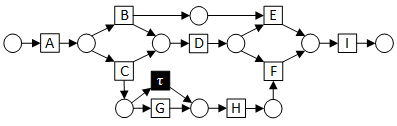
\includegraphics[scale=.5]{fig_BPM/Model_1.png}\bigskip\\
\begin{tabular}{ll}
  Trace & \(\sigma = \sequence{A,B,D,G,H,F,I}\)\\
  Alignment: & \(\gamma = \sequence{A,\alert{C},D,G,H,F,I}\)
\end{tabular}
\end{frame}

\begin{frame}[fragile]{The General Timed Alignment Problem}
\metroset{block=fill}
\begin{block}{GTAP}
  Input : A \alert{time} Petri net $N$ and an observed \alert{timed} trace $\sigma$.
  \medskip\\
  Output : A full \alert{timed} trace $\gamma \in \mathcal{L}(N)$ which minimizes
  its distance to $\sigma$,
  for some distance function $d$ on timed words.
\end{block}
\vfill

\adjustbox{scale=0.7}{	
\begin{tikzcd}
	& {} & \Huge\bigcirc & {\fbox{ec}} & \Huge\bigcirc & {} && {\fbox{pay}} \\
	\Huge\bigcirc & {\fbox{reg}} && {\fbox{et}} && {\fbox{dec}} & \Huge\bigcirc & {} & \Huge\bigcirc \\
	&& \Huge\bigcirc & {\fbox{ct}} & \Huge\bigcirc &&& {\fbox{rej}}
	\arrow["{[0, 1]}"{description, pos=0.2}, shift left=3, draw=white, from=2-2, to=1-2]
	\arrow[""{name=0, anchor=center, inner sep=0}, "{[2,2]}"{description, pos=0.1}, draw=white, from=2-4, to=1-4]
	\arrow["{[2,2]}"{description, pos=0.1}, draw=white, from=3-4, to=2-4]
	\arrow["{[2,4]}"{description, pos=0.1}, shift right=4, draw=white, from=2-6, to=1-6]
	\arrow["{[0,1]}"{description, pos=0.1}, draw=white, from=1-8, to=2-8]
	\arrow["{[0,0]}"{description, pos=0.1}, draw=white, from=3-8, to=2-8]
	\arrow[from=2-1, to=2-2]
	\arrow[curve={height=-12pt}, from=2-2, to=1-3]
	\arrow[curve={height=12pt}, from=2-2, to=3-3]
	\arrow[from=1-3, to=1-4]
	\arrow[from=1-4, to=1-5]
	\arrow[curve={height=12pt}, from=1-3, to=2-4]
	\arrow[curve={height=12pt}, from=2-4, to=1-5]
	\arrow[from=3-3, to=3-4]
	\arrow[from=3-4, to=3-5]
	\arrow[curve={height=-12pt}, from=1-5, to=2-6]
	\arrow[curve={height=12pt}, from=3-5, to=2-6]
	\arrow[from=2-6, to=2-7]
	\arrow[curve={height=-12pt}, from=2-7, to=1-8]
	\arrow[curve={height=12pt}, from=2-7, to=3-8]
	\arrow[curve={height=12pt}, from=3-8, to=2-9]
	\arrow[curve={height=-12pt}, from=1-8, to=2-9]
	\arrow["{[0,2]}"{description, pos=0.2}, draw=white, from=1-4, to=0]
\end{tikzcd}
}
\vfill 
\begin{tabular}{l}
  Trace: \alert{$\sigma = (reg, 1) \cdot (ec, 2) \cdot (ec, 2) \cdot (ct, 3) \cdot (dec, 8) \cdot (rej, 8)$}\medskip\\
  Alignment? \alert{$\gamma_1 = (reg, 1) \cdot (ec, 2) \cdot (ct, 3) \cdot (dec, 7) \cdot (rej, 7)$}\\
  Alignment? \alert{$\gamma_2 = (reg, 1) \cdot (ec, 2) \cdot (ct, 3) \cdot (dec, 7) \cdot (pay, 8)$}\\
\end{tabular}
\end{frame}

\begin{frame}[fragile]{The Purely Timed Alignment Problem}
  \metroset{block = fill}
  \begin{block}{PTAP}
    Input : A time Petri net $N$ and an observed timed trace
    $\sigma = (w_1, \theta_1) \dots (w_n, \theta_n)$
    such that $w$ is a valid untimed trace of \(N\).
    \medskip\\
    Output : A timing function $\eta$ such that
    $\gamma = (w_1, \eta_1) \dots (w_n, \eta_n)$ is a full timed trace of $N$
    and minimizes $d(\theta, \eta)$
    for some distance function $d$ on timing functions.
  \end{block}
\adjustbox{scale=0.7}{	
\begin{tikzcd}
	& {} & \Huge\bigcirc & {\fbox{ec}} & \Huge\bigcirc & {} && {\fbox{pay}} \\
	\Huge\bigcirc & {\fbox{reg}} && {\fbox{et}} && {\fbox{dec}} & \Huge\bigcirc & {} & \Huge\bigcirc \\
	&& \Huge\bigcirc & {\fbox{ct}} & \Huge\bigcirc &&& {\fbox{rej}}
	\arrow["{[0, 1]}"{description, pos=0.2}, shift left=3, draw=white, from=2-2, to=1-2]
	\arrow[""{name=0, anchor=center, inner sep=0}, "{[2,2]}"{description, pos=0.1}, draw=white, from=2-4, to=1-4]
	\arrow["{[2,2]}"{description, pos=0.1}, draw=white, from=3-4, to=2-4]
	\arrow["{[2,4]}"{description, pos=0.1}, shift right=4, draw=white, from=2-6, to=1-6]
	\arrow["{[0,1]}"{description, pos=0.1}, draw=white, from=1-8, to=2-8]
	\arrow["{[0,0]}"{description, pos=0.1}, draw=white, from=3-8, to=2-8]
	\arrow[from=2-1, to=2-2]
	\arrow[curve={height=-12pt}, from=2-2, to=1-3]
	\arrow[curve={height=12pt}, from=2-2, to=3-3]
	\arrow[from=1-3, to=1-4]
	\arrow[from=1-4, to=1-5]
	\arrow[curve={height=12pt}, from=1-3, to=2-4]
	\arrow[curve={height=12pt}, from=2-4, to=1-5]
	\arrow[from=3-3, to=3-4]
	\arrow[from=3-4, to=3-5]
	\arrow[curve={height=-12pt}, from=1-5, to=2-6]
	\arrow[curve={height=12pt}, from=3-5, to=2-6]
	\arrow[from=2-6, to=2-7]
	\arrow[curve={height=-12pt}, from=2-7, to=1-8]
	\arrow[curve={height=12pt}, from=2-7, to=3-8]
	\arrow[curve={height=12pt}, from=3-8, to=2-9]
	\arrow[curve={height=-12pt}, from=1-8, to=2-9]
	\arrow["{[0,2]}"{description, pos=0.2}, draw=white, from=1-4, to=0]
\end{tikzcd}
}	
	
\vfill 
\begin{tabular}{ll}
  Trace: & \alert{$\sigma = (reg, 1) \cdot (ec, 2) \cdot (ct, 3) \cdot (dec, 8) \cdot (rej, 8)$}\\\medskip
  Alignment: & \alert{$\gamma = (reg, 1) \cdot (ec, 2) \cdot (ct, 3) \cdot (dec, 7) \cdot (rej, 7)$}\\
\end{tabular}
\end{frame}

\subsection{Distances}
\begin{frame}{Distances between traces}
    \begin{itemize}
        \item Untimed Alignments : Levenshtein's edit distance 
        \vfill 
        \item \alert{What are meaningful edit moves over timestamp series?}
        \vfill 
    \end{itemize}
\end{frame}

\begin{frame}{Edit Moves}
	Consider a time series, \alert{$$\sigma = (1, 2, 10, 14, 15)$$}
	
    $$\alert{stamp(+5, 2)}\sigma = (1, \alert{7}, 10, 14, 15)$$
\vfill 
Cost : $|+5|$.
	\pause 
	\vfill 
    $$\alert{delay(+5, 2)}\sigma = (1, \alert{7, 15, 19, 20})$$
\vfill 
Cost : $|+5|$.

\end{frame}

\begin{frame}[fragile]{Delay Edit : Branching example}

\adjustbox{scale=0.7}{
\begin{tikzcd}
	& {} & \Huge\bigcirc & {\fbox{ec}} & \Huge\bigcirc & {} && {\fbox{pay}} \\
	\Huge\bigcirc & {\fbox{reg}} && {\fbox{et}} && {\fbox{dec}} & \Huge\bigcirc & {} & \Huge\bigcirc \\
	&& \Huge\bigcirc & {\fbox{\alert{ct}}} & \Huge\bigcirc &&& {\fbox{rej}}
	\arrow["{[0, 1]}"{description, pos=0.2}, shift left=3, draw=white, from=2-2, to=1-2]
	\arrow[""{name=0, anchor=center, inner sep=0}, "{[2,2]}"{description, pos=0.1}, draw=white, from=2-4, to=1-4]
	\arrow["{[2,2]}"{description, pos=0.1}, draw=white, from=3-4, to=2-4]
	\arrow["{[2,4]}"{description, pos=0.1}, shift right=4, draw=white, from=2-6, to=1-6]
	\arrow["{[0,1]}"{description, pos=0.1}, draw=white, from=1-8, to=2-8]
	\arrow["{[0,0]}"{description, pos=0.1}, draw=white, from=3-8, to=2-8]
	\arrow[from=2-1, to=2-2]
	\arrow[curve={height=-12pt}, from=2-2, to=1-3]
	\arrow[curve={height=12pt}, from=2-2, to=3-3]
	\arrow[from=1-3, to=1-4]
	\arrow[from=1-4, to=1-5]
	\arrow[curve={height=12pt}, from=1-3, to=2-4]
	\arrow[curve={height=12pt}, from=2-4, to=1-5]
	\arrow[from=3-3, to=3-4]
	\arrow[from=3-4, to=3-5]
	\arrow[curve={height=-12pt}, from=1-5, to=2-6]
	\arrow[curve={height=12pt}, from=3-5, to=2-6]
	\arrow[from=2-6, to=2-7]
	\arrow[curve={height=-12pt}, from=2-7, to=1-8]
	\arrow[curve={height=12pt}, from=2-7, to=3-8]
	\arrow[curve={height=12pt}, from=3-8, to=2-9]
	\arrow[curve={height=-12pt}, from=1-8, to=2-9]
	\arrow["{[0,2]}"{description, pos=0.2}, draw=white, from=1-4, to=0]
\end{tikzcd}
	}
	
	\vfill 
	
	$$\sigma = (reg, 1)\cdot  (ct, 2)  \cdot (ec, 2) \cdot (dec, 6) \cdot (rej, 6)$$
	
	\vfill 
	$$\alert{delay(1, ct)}\sigma = (reg, 1) \cdot (ec, 2) \cdot  \alert{(ct, 3) \cdot (dec, 7) \cdot (rej, 7)}$$
	
	 \vfill 
	Cost : $|1|$
\end{frame}



\begin{frame}{Three distances : Stamp Only Distance ($d_t$)}
\metroset{block=fill}
\begin{block}{Definition}
    \small $$d_t(\tau_1 \rightarrow \tau_2) = \min \{cost(m) | {m \in Stamp^*}, {m(\tau_1) = \tau_2}\}$$
\end{block}
	


$$d_t((0,1,2) \rightarrow (1,3,3)) = |1| + |2| + |1| = 4$$
\vfill 
Essentially Manhattan distance. 
\end{frame}

\begin{frame}{Three distances : Delay Only Distance ($d_\theta$)}
	\metroset{block=fill}
\begin{block}{Definition}
    	\small $$d_\theta(\tau_1 \rightarrow \tau_2) = \min \{cost(m) | {m \in Delay^*}, {m(\tau_1) = \tau_2}\}$$
\end{block}

	
	$$(0,1,2) \xrightarrow{delay(1,1)}(1,2,3) \xrightarrow{delay(1,2)} (1,3,4) \xrightarrow{delay(-1,3)} (1,3,3)$$
	
$$d_\theta((0,1,2) \rightarrow (1,3,3)) = |1| + |1| + |-1| = 3$$

\vfill 
Essentially Manhattan distance on the gaps between consecutive timestamps. 

\end{frame}
\begin{frame}{Three distances : Mixed Moves Distance ($d_m$)}
\metroset{block=fill}
\begin{block}{Definition}
    \small	$$d_m(\tau_1 \rightarrow \tau_2) = \min \{cost(m) | {m \in (Stamp \cup Delay)^*}, {m(\tau_1) = \tau_2}\}$$
\end{block}
	
	
	
	$$(0,1,2) \xrightarrow{delay(1,1)}(1,2,3) \xrightarrow{stamp(1,2)} (1,3,3)$$
	
$$d_m((0,1,2) \rightarrow (1,3,3)) = |1| + |1|  = 2$$

\bigskip
\begin{block}{Properties}
  \begin{itemize}
  \item \(d_m(\tau_1 \rightarrow \tau_2) \leq d_t(\tau_1 \rightarrow \tau_2)\)
  \item \(d_m(\tau_1 \rightarrow \tau_2) \leq d_\theta(\tau_1 \rightarrow \tau_2)\)
  \item \(d_\theta(\tau_1 \rightarrow \tau_2) \leq 2 \times d_t(\tau_1 \rightarrow \tau_2)\)
  \end{itemize}
\end{block}

\end{frame}
\section{Results and algorithms for PTAP}

\begin{frame}[fragile]{Recall PTAP}

With our newly defined distance functions, we set about solving PTAP for each. 
\vfill 

	\metroset{block = fill}
	\begin{block}{PTAP}
    Input : A time Petri net $N$ and an observed timed trace
    $\sigma = (w_1, \theta_1) \dots (w_n, \theta_n)$
    and a valid causal process of the untimed part $w$.
    \medskip\\
    Output : A timing function $\eta$ such that
    $\gamma = (w_1, \eta_1) \dots (w_n, \eta_n)$ is a full timed trace of $N$
    and minimizes $d(\theta, \eta)$
    for some distance function $d$ on timing functions.
	\end{block}
\adjustbox{scale=0.7}{	
\begin{tikzcd}
	& {} & \Huge\bigcirc & {\fbox{ec}} & \Huge\bigcirc & {} && {\fbox{pay}} \\
	\Huge\bigcirc & {\fbox{reg}} && {\fbox{et}} && {\fbox{dec}} & \Huge\bigcirc & {} & \Huge\bigcirc \\
	&& \Huge\bigcirc & {\fbox{ct}} & \Huge\bigcirc &&& {\fbox{rej}}
	\arrow["{[0, 1]}"{description, pos=0.2}, shift left=3, draw=white, from=2-2, to=1-2]
	\arrow[""{name=0, anchor=center, inner sep=0}, "{[2,2]}"{description, pos=0.1}, draw=white, from=2-4, to=1-4]
	\arrow["{[2,2]}"{description, pos=0.1}, draw=white, from=3-4, to=2-4]
	\arrow["{[2,4]}"{description, pos=0.1}, shift right=4, draw=white, from=2-6, to=1-6]
	\arrow["{[0,1]}"{description, pos=0.1}, draw=white, from=1-8, to=2-8]
	\arrow["{[0,0]}"{description, pos=0.1}, draw=white, from=3-8, to=2-8]
	\arrow[from=2-1, to=2-2]
	\arrow[curve={height=-12pt}, from=2-2, to=1-3]
	\arrow[curve={height=12pt}, from=2-2, to=3-3]
	\arrow[from=1-3, to=1-4]
	\arrow[from=1-4, to=1-5]
	\arrow[curve={height=12pt}, from=1-3, to=2-4]
	\arrow[curve={height=12pt}, from=2-4, to=1-5]
	\arrow[from=3-3, to=3-4]
	\arrow[from=3-4, to=3-5]
	\arrow[curve={height=-12pt}, from=1-5, to=2-6]
	\arrow[curve={height=12pt}, from=3-5, to=2-6]
	\arrow[from=2-6, to=2-7]
	\arrow[curve={height=-12pt}, from=2-7, to=1-8]
	\arrow[curve={height=12pt}, from=2-7, to=3-8]
	\arrow[curve={height=12pt}, from=3-8, to=2-9]
	\arrow[curve={height=-12pt}, from=1-8, to=2-9]
	\arrow["{[0,2]}"{description, pos=0.2}, draw=white, from=1-4, to=0]
\end{tikzcd}
}	
	
\vfill 
\begin{tabular}{ll}
  Trace: & \alert{$\sigma = (reg, 1) \cdot (ec, 2) \cdot (ct, 3) \cdot (dec, 8) \cdot (rej, 8)$}\\\medskip
  Alignment: & \alert{$\gamma = (reg, 1) \cdot (ec, 2) \cdot (ct, 3) \cdot (dec, 7) \cdot (rej, 7)$}\\
\end{tabular}
\end{frame}
\begin{frame}{Delay only, $d_\theta$}
    \begin{itemize}
        \item For a large class of nets (extended free choice), a linear-time algorithm! 
        \vfill 
        \item This distance allows a naive, greedy algorithm. 
    \end{itemize}
\end{frame}


\begin{frame}[fragile]{Delay only Alignment}
    
   \adjustbox{scale=0.7}{
\begin{tikzcd}
	& {} & \Huge\bigcirc & {\fbox{ec}} & \Huge\bigcirc & {} && {\fbox{pay}} \\
	\Huge\bigcirc & {\fbox{reg}} && {\fbox{et}} && {\fbox{dec}} & \Huge\bigcirc & {} & \Huge\bigcirc \\
	&& \Huge\bigcirc & {\fbox{{ct}}} & \Huge\bigcirc &&& {\fbox{rej}}
	\arrow["{[0, 1]}"{description, pos=0.2}, shift left=3, draw=white, from=2-2, to=1-2]
	\arrow[""{name=0, anchor=center, inner sep=0}, "{[2,2]}"{description, pos=0.1}, draw=white, from=2-4, to=1-4]
	\arrow["{[2,2]}"{description, pos=0.1}, draw=white, from=3-4, to=2-4]
	\arrow["{[2,4]}"{description, pos=0.1}, shift right=4, draw=white, from=2-6, to=1-6]
	\arrow["{[0,1]}"{description, pos=0.1}, draw=white, from=1-8, to=2-8]
	\arrow["{[0,0]}"{description, pos=0.1}, draw=white, from=3-8, to=2-8]
	\arrow[from=2-1, to=2-2]
	\arrow[curve={height=-12pt}, from=2-2, to=1-3]
	\arrow[curve={height=12pt}, from=2-2, to=3-3]
	\arrow[from=1-3, to=1-4]
	\arrow[from=1-4, to=1-5]
	\arrow[curve={height=12pt}, from=1-3, to=2-4]
	\arrow[curve={height=12pt}, from=2-4, to=1-5]
	\arrow[from=3-3, to=3-4]
	\arrow[from=3-4, to=3-5]
	\arrow[curve={height=-12pt}, from=1-5, to=2-6]
	\arrow[curve={height=12pt}, from=3-5, to=2-6]
	\arrow[from=2-6, to=2-7]
	\arrow[curve={height=-12pt}, from=2-7, to=1-8]
	\arrow[curve={height=12pt}, from=2-7, to=3-8]
	\arrow[curve={height=12pt}, from=3-8, to=2-9]
	\arrow[curve={height=-12pt}, from=1-8, to=2-9]
	\arrow["{[0,2]}"{description, pos=0.2}, draw=white, from=1-4, to=0]
\end{tikzcd}
	}
	\vfill
	Say we want to align  $\sigma = (reg, 1)(et, 2)(ct, 5)(dec, 6)(rej, 8)$ to $N$.
        \pause\bigskip\\
        Consider the delays taken for a faulty ``execution'' guided by \(\sigma\).
        \\
        \uncover<3->{Pick the best values possible for them, naively.}
\vfill 
\adjustbox{scale=0.7}{
\begin{tikzcd}
	& {} & \Huge\bigcirc & {\fbox{ec}} & \Huge\bigcirc & {} && {\fbox{pay}} \\
	\Huge\bigcirc & {\fbox{reg}} && {\fbox{et}} && {\fbox{dec}} & \Huge\bigcirc & {} & \Huge\bigcirc \\
	&& \Huge\bigcirc & {\fbox{{ct}}} & \Huge\bigcirc &&& {\fbox{rej}}
	\arrow["{\alert{1\only<3->{\rightarrow 1}}}"{description, pos=0.2}, shift left=3, draw=white, from=2-2, to=1-2]
	\arrow[""{name=0, anchor=center, inner sep=0}, "{\alert{1\only<3->{\rightarrow 2}}}"{description, pos=0.1}, draw=white, from=2-4, to=1-4]
	\arrow["{\alert{4\only<3->{\rightarrow 2}}}"{description, pos=0.1}, draw=white, from=3-4, to=2-4]
	\arrow["{\alert{1\only<3->{\rightarrow 2}}}"{description, pos=0.1}, shift right=4, draw=white, from=2-6, to=1-6]
%	\arrow["{[0,1]}"{description, pos=0.1}, draw=white, from=1-8, to=2-8]
	\arrow["{\alert{2\only<3->{\rightarrow 0}}}"{description, pos=0.1}, draw=white, from=3-8, to=2-8]
	\arrow[from=2-1, to=2-2]
	\arrow[curve={height=-12pt}, from=2-2, to=1-3]
	\arrow[curve={height=12pt}, from=2-2, to=3-3]
	\arrow[from=1-3, to=1-4]
	\arrow[from=1-4, to=1-5]
	\arrow[curve={height=12pt}, from=1-3, to=2-4]
	\arrow[curve={height=12pt}, from=2-4, to=1-5]
	\arrow[from=3-3, to=3-4]
	\arrow[from=3-4, to=3-5]
	\arrow[curve={height=-12pt}, from=1-5, to=2-6]
	\arrow[curve={height=12pt}, from=3-5, to=2-6]
	\arrow[from=2-6, to=2-7]
	\arrow[curve={height=-12pt}, from=2-7, to=1-8]
	\arrow[curve={height=12pt}, from=2-7, to=3-8]
	\arrow[curve={height=12pt}, from=3-8, to=2-9]
	\arrow[curve={height=-12pt}, from=1-8, to=2-9]
%	\arrow["{[0,2]}"{description, pos=0.2}, draw=white, from=1-4, to=0]
\end{tikzcd}
	}\\\pause\pause
	From which we reconstruct the closest $\gamma = (reg, 1)(et, 3)(ct, 3)(dec, 5)(rej, 5)$.
\end{frame}

\begin{frame}{Stamp only, $d_t$}
	\begin{itemize}

		\item In general for bounded nets, we have an encoding as an LPP. 
		\vfill 
		%% \item Does not mesh well with the semantics of time Petri nets, small local changes can have bad overall effects.
		%% \vfill 
		\item For sequential causal processes, a direct quadratic time algorithm! 
		\vfill 
	\end{itemize}
\end{frame}



\begin{frame}[fragile]{Stamp only Alignment}
	
\adjustbox{scale=0.7}{
\begin{tikzcd}
	& {} && {} && {} && {\fbox{\alert{pay}}} \\
	\Huge\bigcirc & {\fbox{\alert{reg}}} & \Huge\bigcirc & {\fbox{\alert{check}}} & \Huge\bigcirc & {\fbox{\alert{dec}}} & \Huge\bigcirc & {} & \Huge\bigcirc \\
	&&&&&&& {\fbox{rej}}
	\arrow["{[0, 1]}"{description, pos=0.2}, draw=white, from=2-2, to=1-2]
	\arrow["{[0,1]}"{description, pos=0.2}, draw=white, from=1-8, to=2-8]
	\arrow["{[0,0]}"{description, pos=0.2}, draw=white, from=3-8, to=2-8]
	\arrow[from=2-1, to=2-2]
	\arrow[from=2-2, to=2-3]
	\arrow[from=2-3, to=2-4]
	\arrow[from=2-4, to=2-5]
	\arrow[from=2-5, to=2-6]
	\arrow[from=2-6, to=2-7]
	\arrow[curve={height=-12pt}, from=2-7, to=1-8]
	\arrow[curve={height=12pt}, from=2-7, to=3-8]
	\arrow[curve={height=12pt}, from=3-8, to=2-9]
	\arrow[curve={height=-12pt}, from=1-8, to=2-9]
	\arrow["{[2,4]}"{description, pos=0.2}, draw=white, from=2-6, to=1-6]
	\arrow["{[2,2]}"{description, pos=0.2}, draw=white, from=2-4, to=1-4]
\end{tikzcd}
	}
	\vfill 

\begin{tabular}{cl}
  Trace:
  & $\sigma = \alert{(reg, 1)\cdot (check, 2) \cdot (dec, 4) \cdot (pay, 6)}$\\\\
  Optimal alignments\pause
  & $\gamma = \alert{(reg, 0)\cdot (check, 2) \cdot (dec, 4) \cdot (pay, 5)}$\\
  (examples):
  & $\gamma = \alert{(reg, 1)\cdot (check, 3) \cdot (dec, 5) \cdot (pay, 6)}$\medskip\\
  & Alignment cost: \(d_t(\sigma, \gamma) = 2\)
\end{tabular}
\bigskip\pause
\definecolor{Brickred}{RGB}{200,60,60}       
\setbeamercolor{block title alerted}{%
    use={block title, alerted text},
    fg = Brickred}
    
 \setbeamercolor{block body alerted}{%
    use={block body, alerted text},
    fg = Brickred}   
\begin{alertblock}{How to compute them?}
\end{alertblock}
\end{frame}


\begin{frame}{Stamps Only}
 %% \begin{tabular}{cl}  
 %%         \begin{tabular}{c}
 %%         \parbox{0.45\linewidth}{       We first find the minimum cost $\alert{c}$ of aligning the log trace $\sigma$ to $N$, and then backtrack to find the model trace $\gamma_t$.
 %%    }
 %%           \end{tabular}
 %%           & \begin{tabular}{l}
  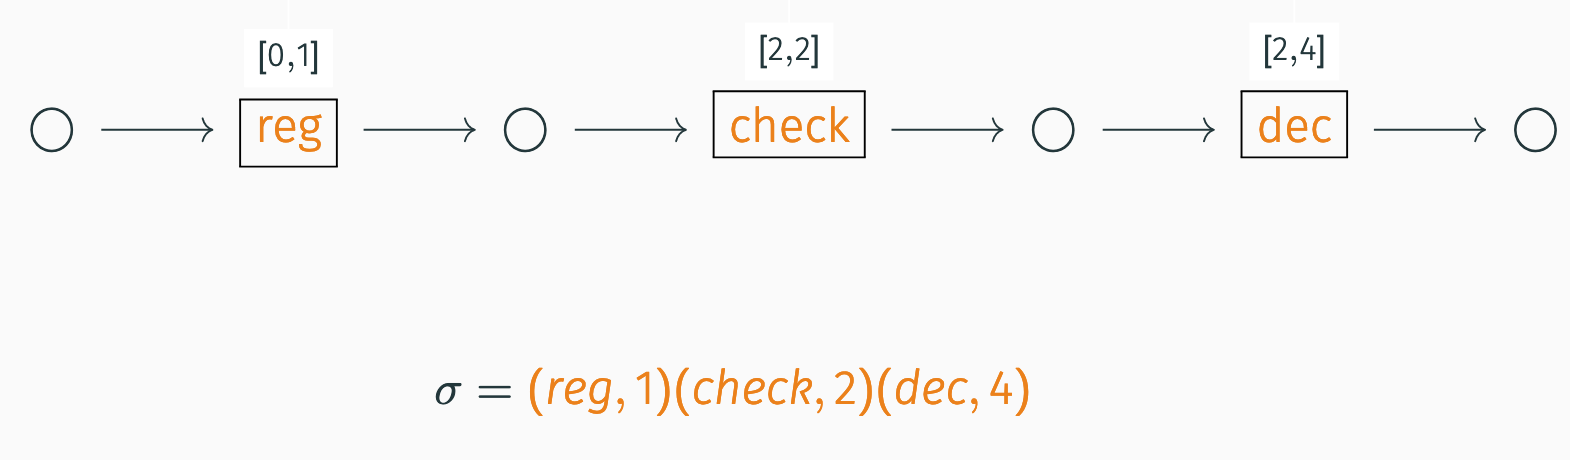
\includegraphics[width=10cm]{n3.png}
%%              \end{tabular}
    
%%     \end{tabular}
%%     $$cost(\gamma) = \sum_{i = 1}^{n}{|\gamma_i - \sigma_i|}$$
%%         \vfill 
%% %        
%% %         
%% %  change the parbox width as appropriate
  \bigskip
  Define \emph{$g_i(d)$} the minimum cost of aligning the $i$-length prefix \(\sigma_1 \dots \sigma_i\) to any \(\gamma_1 \dots \gamma_i \in \mathcal{L}^i(N)\), with the constraint that the timestamp of \(\gamma_i\) should be \(d\).

       %% $$g_i(d) = \min_{\tau|_i \in \mathcal{L}^i(N) \wedge \tau_i = d} cost(\tau|_i)$$ 
\end{frame}

\begin{frame}{Example}
\begin{tabular}{cl}
  \begin{tabular}{c}
    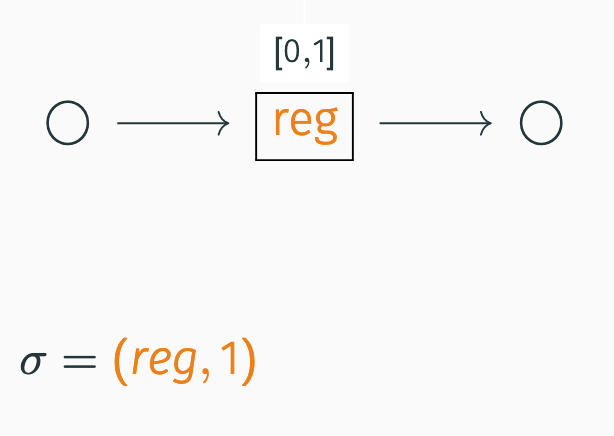
\includegraphics[width=4cm]{n1.png}
  \end{tabular}
  & \begin{tabular}{l}
      \parbox{0.4\linewidth}{%  change the parbox width as appropriate
        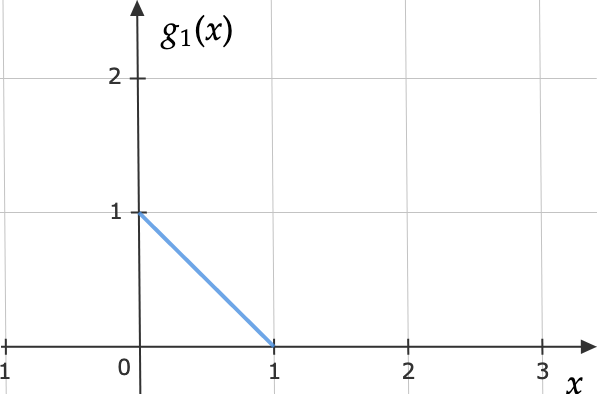
\includegraphics[width=5cm]{g1.png}
    }\end{tabular}
    
    \end{tabular}
             \vfill 
             $$g_1(d) = d_t(\alert{(reg,d) \to (reg,1)}) = |d - 1| = |d-\sigma_1|$$

    \end{frame}
    
    \begin{frame}{Stamp only algorithm for sequential models, continued}

 

        Split cost at the last letter to get the following recursion : 
        	%$$\min_{\tau|_{i+1} \in \mathcal{L}^{i+1}(N)}cost(\tau|_{i+1}) = \min_{\tau_{i+1} - \tau_i\in [a, b]} (|\tau_{i+1} - \sigma_{i+1}| + \min_{\tau|_i \in \mathcal{L}^i(N) }cost(\tau|_i))$$
        	$$g_{i+1}(d) = |d - \sigma_{i+1}| + \min_{d-d' \in [a,b]} g_i(d')$$
        	
        	 
        		
\begin{tabular}{cl}  
         \begin{tabular}{c}
        
           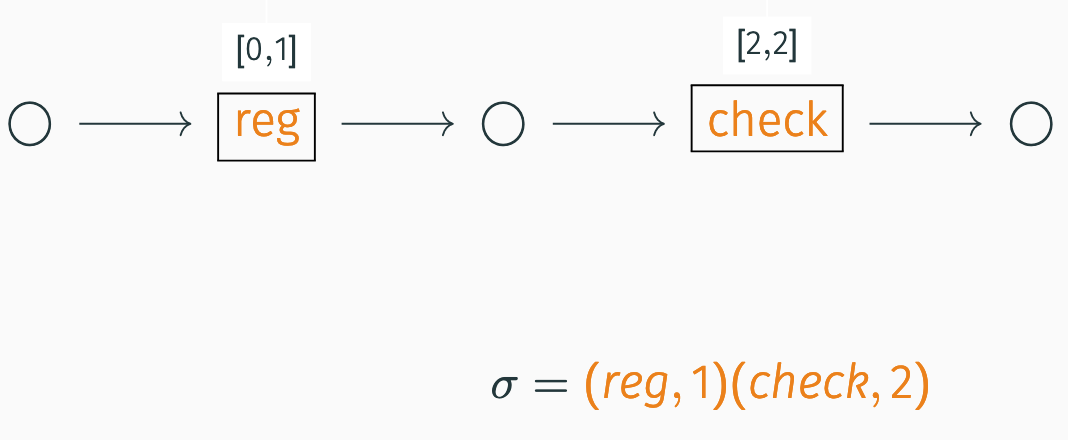
\includegraphics[width=5cm]{n2.png}
           
           \end{tabular}
           & \begin{tabular}{l}
             \parbox{0.4\linewidth}{%  change the parbox width as appropiate
  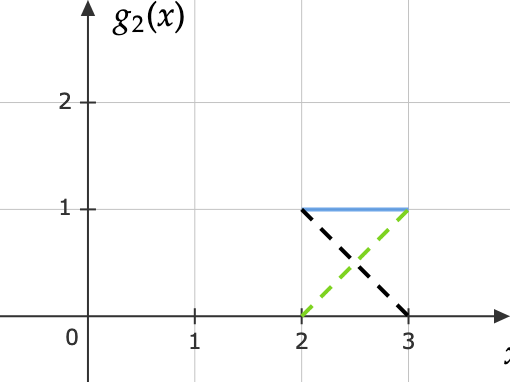
\includegraphics[width=4cm]{g2.png}
    }\end{tabular}
    
    \end{tabular}     
    
   $d_t(\alert{(reg,d-2)(check,d) \to (reg,1)(check,2)}) =$
   
   $g_2(d) = |d-2| + (g_1(d-2))$

    \end{frame}

%\begin{frame}[fragile]{Stamp only : Example}
%	Recall the process model $N$ : 
%		\\
%			\adjustbox{scale=0.6}{
%		\begin{tikzcd}
%	& {} && {} && {} && {\fbox{pay}} \\
%	\Huge\bigcirc & {\fbox{reg}} & \Huge\bigcirc & {\fbox{check}} & \Huge\bigcirc & {\fbox{dec}} & \Huge\bigcirc & {} & \Huge\bigcirc \\
%	&&&&&&& {\fbox{rej}}
%	\arrow["{[0, 1]}"{description, pos=0.2}, draw=white, from=2-2, to=1-2]
%	\arrow["{[0,1]}"{description, pos=0.1}, draw=white, from=1-8, to=2-8]
%	\arrow["{[0,0]}"{description, pos=0.1}, draw=white, from=3-8, to=2-8]
%	\arrow[from=2-1, to=2-2]
%	\arrow[from=2-2, to=2-3]
%	\arrow[from=2-3, to=2-4]
%%%%	\arrow[curve={height=-12pt}, from=2-7, to=1-8]
%	\arrow[curve={height=12pt}, from=2-7, to=3-8]
%	\arrow[curve={height=12pt}, from=3-8, to=2-9]
	%\arrow[curve={height=-12pt}, from=1-8, to=2-9]
	%\arrow["{[2,4]}"{description}, draw=white, from=2-6, to=1-6]
	%\arrow["{[2,2]}"{description, pos=0.2}, draw=white, from=2-4, to=1-4]
%\end{tikzcd}}

%\vfill 
%		The observed trace is $$\sigma = (reg, 1)\cdot (check, 2) \cdot (dec, 4) \cdot (pay, 6)$$
%		\vfill 
%        In the ith graph, the colour key is \textcolor{blue}{$g_i(d)$}, \textcolor{orange}{$\min_{d-d' \in [a,b]}$} $g_{i-1}(d')$, and \textcolor{green}{$|d - \sigma_i|$}
%\end{frame}

% \begin{frame}{ Diagrams: $g_1, g_2$}
%        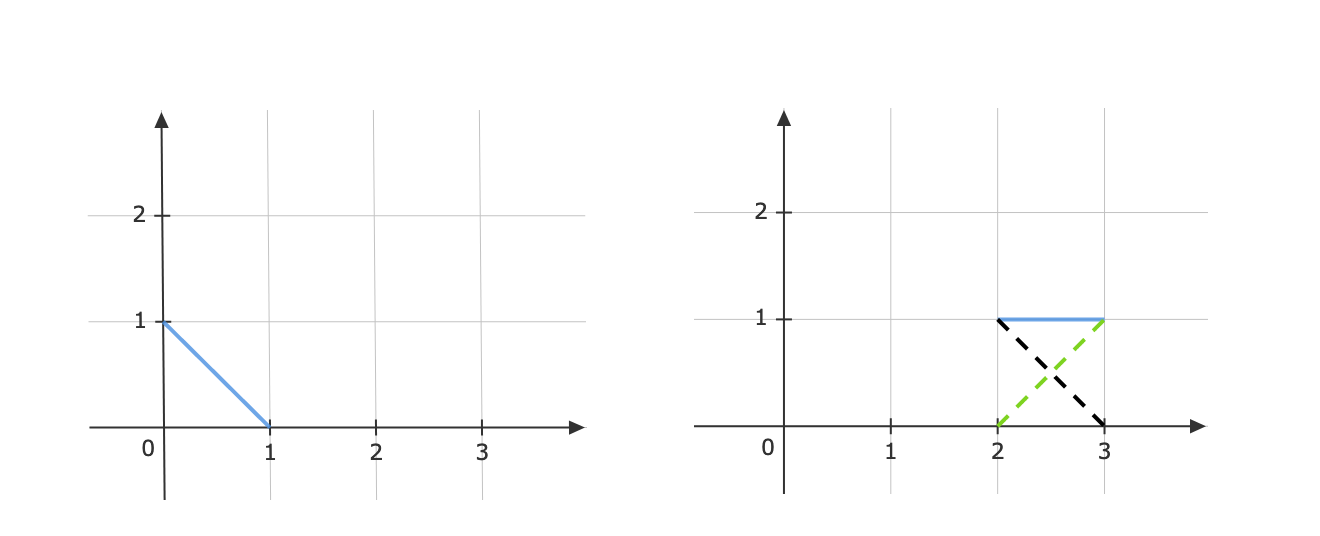
\includegraphics[width = \textwidth]{g12.png}
%\end{frame}

\begin{frame}[fragile]{Diagrams: $g_3, g_4$}
               In the ith graph, the colour key is \textcolor{blue}{$g_i(d)$}, \textcolor{orange}{$\min_{d-d' \in [a,b]}$} $g_{i-1}(d')$, and \textcolor{green}{$|d - \sigma_i|$}
               \vfill 
               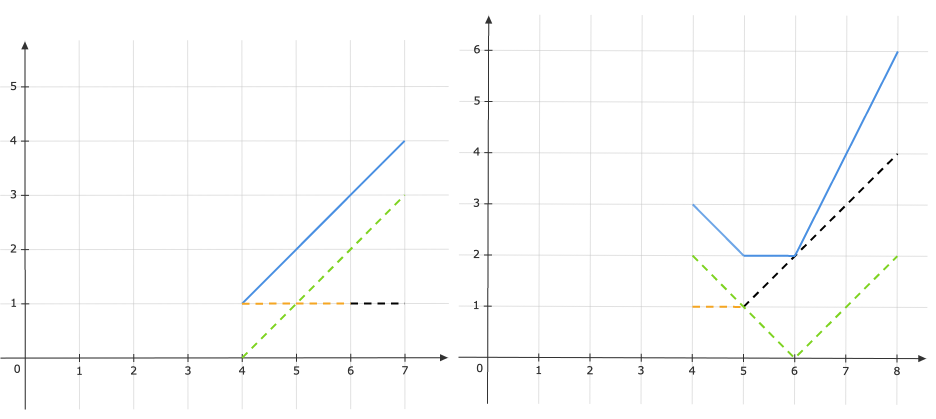
\includegraphics[width = .8\textwidth]{g34.png}
	
\adjustbox{scale=0.7}{
\begin{tikzcd}
	& {} && {} && {} && {} \\
	\Huge\bigcirc & {\fbox{\alert{reg}}} & \Huge\bigcirc & {\fbox{\alert{check}}} & \Huge\bigcirc & {\fbox{\alert{dec}}} & \Huge\bigcirc & {\fbox{\alert{pay}}} & \Huge\bigcirc \\
	&&&&&&& {}
	\arrow["{[0,1]}"{description, pos=0.2}, draw=white, from=2-2, to=1-2]
	\arrow["{[0,1]}"{description, pos=0.2}, draw=white, from=2-8, to=1-8]
	\arrow[from=2-1, to=2-2]
	\arrow[from=2-2, to=2-3]
	\arrow[from=2-3, to=2-4]
	\arrow[from=2-4, to=2-5]
	\arrow[from=2-5, to=2-6]
	\arrow[from=2-6, to=2-7]
	\arrow[from=2-7, to=2-8]
	\arrow[from=2-8, to=2-9]
	\arrow["{[2,4]}"{description, pos=0.2}, draw=white, from=2-6, to=1-6]
	\arrow["{[2,2]}"{description, pos=0.2}, draw=white, from=2-4, to=1-4]
\end{tikzcd}
	}
	\vfill 

\begin{tabular}{cl}
  Trace:
  & $\sigma = \alert{(reg, 1)\cdot (check, 2) \cdot (dec, 4) \cdot (pay, 6)}$\\\\
  Optimal alignments
  & $\gamma = \alert{(reg, 0)\cdot (check, 2) \cdot (dec, 4) \cdot (pay, 5)}$\\
  (examples):
  & $\gamma = \alert{(reg, 1)\cdot (check, 3) \cdot (dec, 5) \cdot (pay, 6)}$
\end{tabular}
\end{frame}

\begin{frame}{Summary: Algorithm for Stamp only Alignment}
  \begin{itemize}
  \item Compute the \(g_i\)'s incrementally
  \item Store them as lists of segments
    \begin{itemize}
    \item no more than \(i\) segments for \(g_i\)
    \item slopes of \(g_i\) segments are integers in \([-i, i]\)
    \end{itemize}
    \(\rightarrow O(n^2)\) time
  \item The minimum cost of alignment is $c = \min_{d} g_n(d)$.
    \bigskip
  \item Reconstruct an optimal alignment \(\gamma\):
    \begin{itemize}
    \item Pick some \(d\) which minimizes the cost \(g_n(d)\), \(d\) is the
      timestamp of \(\gamma_n\)
    \item Then backtrack to get the timestamp of \(\gamma_{n-1}\)
    \item \dots
    \end{itemize}
  \end{itemize}
  \bigskip
  \begin{block}{Implementation in Python}
    Available at \url{https://github.com/NehaRino/TimedAlignments}
  \end{block}
\end{frame}

%\begin{frame}{Mixed moves, $d_m$ : Computation}
%    \begin{itemize}
%        \item Firstly, we have a linear time algorithm for calculating the distance for sequential causal processes 
%        \vfill 
%        \item The algorithm is simple, but the proof of correctness was difficult
%    \end{itemize}
%\end{frame}

%\begin{frame}{Mixed moves, $d_m$ : Alignment}
%\metroset{block=fill}
%\begin{block}{Mixed Moves Alignment Result}
%    $\gamma_N = \gamma_\theta$
%\end{block}
%		\vfill 
%		 This gives us a linear algorithm for aligning under $d_m$, again, proving correctness was the hard part.  
%\end{frame}


\section{Conclusion}
\begin{frame}{Summary of Contributions}
\begin{itemize}
	\item We set the problem of General and Purely Timed Alignment for process models.
	\vfill
	\item We defined three metrics for timed words, and studied the purely timed alignment problem over them.
	\vfill
	\item For certain classes of process models, we provide original and efficient algorithms to solve purely timed alignment
          \begin{itemize}
          \item Quadratic time for Stamp only Alignment
          \item Linear time for Mixed moves Alignment
          \end{itemize}

\end{itemize}
\end{frame}

\begin{frame}[fragile]{Future Directions : Back to GTAP}
  \begin{itemize}
  \item \adjustbox{scale=0.6}{
      \begin{tikzcd}
	& {} && {} && {} && {\fbox{pay}} \\
	\Huge\bigcirc & {\fbox{reg}} & \Huge\bigcirc & {\fbox{check}} & \Huge\bigcirc & {\fbox{dec}} & \Huge\bigcirc & {} & \Huge\bigcirc \\
	&&&&&&& {\fbox{rej}}
	\arrow["{[0, 1]}"{description, pos=0.2}, draw=white, from=2-2, to=1-2]
	\arrow["{\alert{[0,1]}}"{description, pos=0.1}, draw=white, from=1-8, to=2-8]
	\arrow["{\alert{[1000,1000]}}"{description, pos=0.1}, draw=white, from=3-8, to=2-8]
	\arrow[from=2-1, to=2-2]
	\arrow[from=2-2, to=2-3]
	\arrow[from=2-3, to=2-4]
	\arrow[from=2-4, to=2-5]
	\arrow[from=2-5, to=2-6]
	\arrow[from=2-6, to=2-7]
	\arrow[curve={height=-12pt}, from=2-7, to=1-8]
	\arrow[curve={height=12pt}, from=2-7, to=3-8]
	\arrow[curve={height=12pt}, from=3-8, to=2-9]
	\arrow[curve={height=-12pt}, from=1-8, to=2-9]
	\arrow["{[2,4]}"{description}, draw=white, from=2-6, to=1-6]
	\arrow["{[2,2]}"{description, pos=0.2}, draw=white, from=2-4, to=1-4]
    \end{tikzcd}}
    \vfill
  \item Approach 1 : First align actions, then timestamps
    \vfill
  \item Consider : $\sigma = (reg, 0)(check, 2)(dec, 4)\alert{(pay, 1004)}$
    \vfill
  \item Approach 1 is quite biased towards actions, but it is a start.
    \vfill
  \item Approach 2 : set a cost for action edits.
  \end{itemize}
\end{frame}


\begin{frame}{Future Directions : Other Conformance checking artefacts for time-aware systems}
  \bigskip
  \scalebox{.7}{\begin{tabular}{l}
    $\langle A,B,D,E,I \rangle$    \\
    $\langle A,C,D,G,H,F,I \rangle$  \\
    $\langle A,C,G,D,H,F,I \rangle$  \\
    $\langle A,C,H,D,F,I \rangle$    \\
    $\langle A,C,D,H,F,I \rangle$    \\
  \end{tabular}}
  \hfill\(\longrightarrow\)\hfill
  \raisebox{-.8cm}{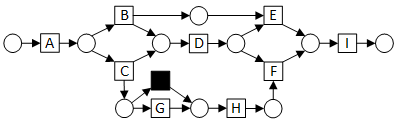
\includegraphics[width=5cm]{model_Boudewijn.png}}
  %% \\\hspace*{0.8\textwidth}{\Huge ?}
  \bigskip
  \begin{block}{Quality criteria to evaluate models}
    \begin{itemize}
    \item $\model$ \emph{fits} $\logs$ if $\logs \subseteq \Language(\model)$
    \item $\model$ is \emph{precise} if its runs are \textit{close} to traces of $\logs$
    \item $\model$ \emph{generalizes} $\logs$ %% with respect to ${\sys}$
      if $\Language(\model)$ contains some unobserved behavior $\not\in
      %% in $\Language(\sys) \backslash
      \logs$
    \item \emph{simplicity}\dots
    %% \item fitness
    %% \item \emph{precision}
    %% \item simplicity
    %% \item generalization
    \end{itemize}
  \end{block}
  \bigskip
  \alert{Alignments} are central for measuring \emph{fitness}
  \medskip\\\pause
  \alert{Anti-alignments} are used to measure \emph{precision}.
  \begin{itemize}
  \item PhD thesis of Mathilde Boltenhagen
  \end{itemize}
\end{frame}

\begin{frame}{Anti-alignments -- Motivation}
  \emph{Estimating precision}\\
  A model is \emph{precise} if it produces only traces which are \textit{close}
  to log traces.
  \bigskip

  Log \(L\):\smallskip\\
  \raisebox{.8cm}{\(\Ar{l}{
      \sequence{A,C,D,G,H,F,I}\\
      \sequence{A,C,G,D,H,F,I}\\
      \sequence{A,C,D,H,F,I}\\
      \sequence{A,C,H,D,F,I}\\
    }\)}
  \hfill
  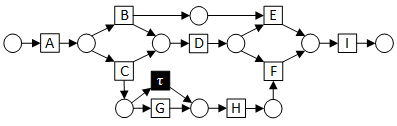
\includegraphics[scale=.5]{fig_BPM/Model_1.png}\bigskip\\
  \bigskip

  \begin{block}{Motivation}
    In order to measure precision, find the run of \(N\) which is most \emph{misaligned}
    with the log \(L\).
  \end{block}
  \bigskip\pause
  \alert{Here: \(\sequence{A,B,D,E,I}\)}
\end{frame}

\begin{frame}{Anti-alignments -- Results}
  \begin{block}{Precision metric based on anti-alignements \cite{ICATPN'2016, BPM'2016, ICPM'2021, Inf. Systems'2021}}
    \begin{itemize}
    \item Anti-alignment serves as witness for \textit{im}precision
    \item Precision metric verifies properties of {\small [Tax et al., IPL 2018]}
    \item Several implementations: SAT encoding, then very efficient approximations (discounted edit distance)
    \end{itemize}
  \end{block}
  \bigskip
\definecolor{Brickred}{RGB}{200,60,60}       
\setbeamercolor{block title alerted}{%
    use={block title, alerted text},
    fg = Brickred}
    
 \setbeamercolor{block body alerted}{%
    use={block body, alerted text},
    fg = Brickred}   
  \begin{alertblock}
    {\Large Anti-alignments for timed models?}
  \end{alertblock}
\end{frame}


\begin{frame}{Future Directions (again!)}
  \emph{Conformance checking}
  \begin{itemize}
  \item Take into account
    \begin{itemize}
    \item time information
    \item other quantitative information (cost, mark)
    \end{itemize}
  \item \emph{Entropy} of timed model (vs. entropy computed from the log)
  \end{itemize}
  \bigskip

  \emph{Model repair}
  \begin{itemize}
  \item How to modify/edit a model incrementally in order to improve its
    quality?
  \end{itemize}
  \bigskip

  \emph{Stochastic models} to represent frequencies of observed traces
  \begin{itemize}
  \item hot topic in Process Mining currently, but very delicate IMO
  \end{itemize}
  \bigskip

  \emph{Comparison of models}
  \begin{itemize}
  \item Spot differences between several models of the same process
  \end{itemize}
  \bigskip

  \emph{Expressiveness of formalisms/classes of models, e.g. BPMN vs. Petri nets}

\end{frame}



\begin{frame}
    \Huge{\centerline{\textbf{Thank you!}}}
\end{frame}


%\appendix





%\begin{frame}{Mixed Moves Alignment}
	
%	Let us try to align the observed trace $(0, 3, 4)$ to the process trace $(0.5, 2.5, 3.5)$ under $d_m$

%\vfill 
%Intuitively,  we can assume a minimum cost run is left to right, or, \alert{chronological}. 
%\vfill 
%So our first move will have to incur a minimum cost of $0.5$ as we try to align $(0,3,4)$ to our process trace at the first position.
%\vfill 
%Ensuring a move is not counterproductive at a position is what we call \alert{co-operation}. 


%\end{frame} 

%\begin{frame}{Mixed Moves Alignment}

%	Now we move on to move two, which will again incur a minimum cost of $0.5$. 
%	\vfill 
%	This unique choice of stamp that moves the local component as close as possible to the desired one indirectly represents what we define as \alert{stability}. 
%	\vfill 
%	Hence, the least cost alignment is $(0.5, 0, 1)(0, -0.5, 2)$, with total cost 1. 
%	\vfill 
%	In fact distance 1 is the best we can do here even in the mixed case. 
%\end{frame} 
%----------------------------------------------------------------------------------------



\end{document}
